\documentclass[a4paper,12pt]{article}
\usepackage[utf8]{inputenc}
\usepackage[spanish]{babel}
\usepackage{color}
\usepackage{parskip}
\usepackage{graphicx}
\usepackage{multirow}
\usepackage{listings}
\usepackage{vmargin}
\usepackage{datetime}
\newdate{date}{14}{12}{2017}
\graphicspath{ {imagenes/} }
\definecolor{mygreen}{rgb}{0,0.6,0}
\definecolor{lbcolor}{rgb}{0.9,0.9,0.9}
\usepackage{epstopdf}
\usepackage{float}


\setpapersize{A4}
\setmargins{2.5cm}       % margen izquierdo
{1.5cm}                        % margen superior
{16.5cm}                      % anchura del texto
{23.42cm}                    % altura del texto
{10pt}                           % altura de los encabezados
{1cm}                           % espacio entre el texto y los encabezados
{0pt}                             % altura del pie de página
{2cm}     

\lstset{
    tabsize=4,    
%   rulecolor=,
    language=[GNU]C++,
        basicstyle=\tiny,
        aboveskip={1.5\baselineskip},
        columns=fixed,
        showstringspaces=false,
        extendedchars=false,
        breaklines=true,
        prebreak = \raisebox{0ex}[0ex][0ex]{\ensuremath{\hookleftarrow}},
        frame=single,
        showtabs=false,
        showspaces=false,
        showstringspaces=false,
        identifierstyle=\ttfamily,
        keywordstyle=\color[rgb]{0,0,1},
        commentstyle=\color[rgb]{0.026,0.112,0.095},
        stringstyle=\color{red},
        numberstyle=\color[rgb]{0.205, 0.142, 0.73},
%        \lstdefinestyle{C++}{language=C++,style=numbers}’.
}


\begin{document}
\title{Laboratorio 7}
\author{
Christofer Fabián Chávez Carazas \\
\small{Universidad Nacional de San Agustín de Arequipa} \\
\small{Escuela Profesional de Ciencia de la Computación} \\
\small{Computación Gráfica}
}
\date{\displaydate{date}}

\maketitle

\begin{enumerate}
 \item \textbf{Copie y analize el siguiente código}
 \begin{itemize}
  \item La función \textit{triangle} dibuja un triangulo a partir de un array de puntos.
  \item \textit{glViewport():} Esta función es para cambiar la ventana de visualización. Se le pasa las coordenada x,y del origen y el tamaño de la ventana.
  \item \textit{glRotatef():} Esta función rota todos los puntos que se van a dibujar debajo. Se le pasa el ángulo de rotación y se le dice por cual eje se quiere rotar.
  \item La función \textit{displayFcn} actualiza la ventana de visualización y luego dibujo un triángulo. Después utiliza la función \textit{glRotatef} y luego dibuja el
  mismo triángulo. El resultado es el triángulo rotado 90 grados.
 \end{itemize}

 \begin{figure}[H]
  \centering
  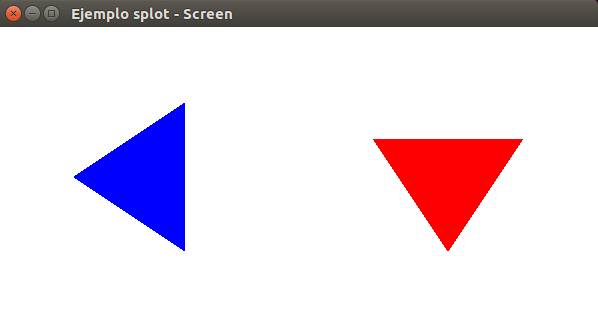
\includegraphics[scale = 0.5]{1.png}
  \caption{Resultados}
 \end{figure}

 \item \textbf{Modifique el código anterior con la finalidad de probar las siguientes transformaciones geométricas de OpenGl:}
 
 \textbf{Sin stack}
 
 \begin{lstlisting}
void displayFcn(){
	glClear(GL_COLOR_BUFFER_BIT);
	glColor3f(0.0,0.0,1.0);
	glRecti(50,100,200,150);
	glColor3f(1.0,0.0,0.0);
	glTranslatef(200, 50, 0);
	glRecti(50,100,200,150);
	glLoadIdentity();
	glRotatef(90.0,0.0,0.0,1.0);
	glTranslatef(70,-600,0);
	glRecti(50,100,200,150);
	glLoadIdentity();
	glScalef(0.5,1.0,1.0);
	glTranslatef(500,-50,0);
	glRecti(50,100,200,150);
	glLoadIdentity();
	glFlush();
}
 \end{lstlisting}

 \textbf{Con stack}
 
 \begin{lstlisting}
void displayFcn(){
	glClear(GL_COLOR_BUFFER_BIT);
	glColor3f(0.0,0.0,1.0);
	glRecti(50,100,200,150);
	glPushMatrix();
	glColor3f(1.0,0.0,0.0);
	glTranslatef(200, 50, 0);
	glRecti(50,100,200,150);
	glPopMatrix();
	glPushMatrix();
	glRotatef(90.0,0.0,0.0,1.0);
	glTranslatef(70,-600,0);
	glRecti(50,100,200,150);
	glPopMatrix();
	glPushMatrix();
	glScalef(0.5,1.0,1.0);
	glTranslatef(500,-50,0);
	glRecti(50,100,200,150);
	glPopMatrix();
	glPushMatrix();
	glFlush();
}
 \end{lstlisting}

 \begin{figure}[H]
  \centering
  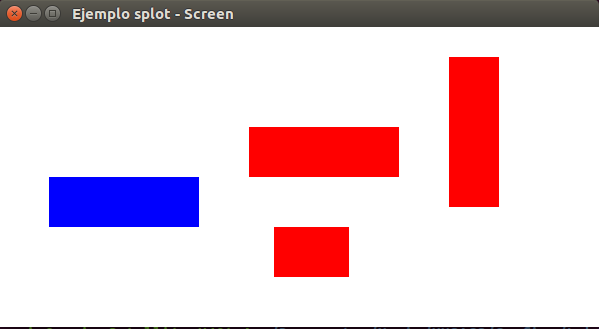
\includegraphics[scale = 0.5]{2.png}
  \caption{Resultados sin stack}
 \end{figure}
 \begin{figure}[H]
  \centering
  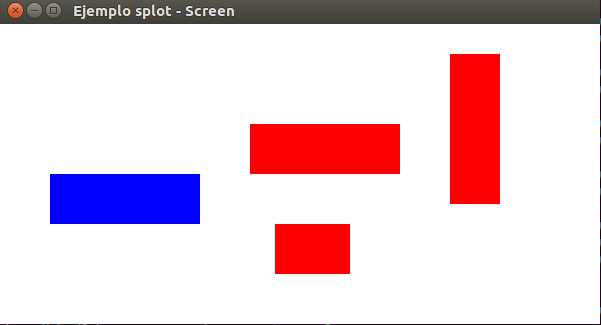
\includegraphics[scale = 0.5]{3.png}
  \caption{Resultados con stack}
 \end{figure}

 \item \textbf{Divida el visor en cuatro zonas, de tal manera que el polígono del primer 
 cuadrante se muestre con diferentes ángulos de rotación}
 
 \begin{enumerate}
  \item \textbf{Utilizando las funciones OpenGL}

 \begin{lstlisting}
#include <GL/glut.h>

class wcPt2D{
public:
	GLfloat x,y;
};

void init(){
	glClearColor(1.0,1.0,1.0,1.0);
	glMatrixMode(GL_PROJECTION);
	gluOrtho2D(-100.0,100.0,-100.0,100.0);
	glMatrixMode(GL_MODELVIEW);
}

void triangle(wcPt2D * verts){
	GLint k;
	glBegin(GL_TRIANGLES);
		for(k = 0; k < 3; k++){
			glVertex2f(verts[k].x, verts[k].y);
		}
	glEnd();
}

void displayFcn(){
	wcPt2D verts[3] = {{-50, 50}, {50,50}, {0.0,-25}};
	glClear(GL_COLOR_BUFFER_BIT);
	glColor3f(0.0,0.0,1.0);
	glViewport(0,300,300,300);
	triangle(verts);
	glViewport(0,0,300,300);
	glRotatef(90.0,0.0,0.0,1.0);
	triangle(verts);
	glViewport(300,0,300,300);
	glRotatef(90.0,0.0,0.0,1.0);
	triangle(verts);
	glViewport(300,300,300,300);
	glRotatef(90.0,0.0,0.0,1.0);
	triangle(verts);
	glFlush();
}

int main(int argc, char ** argv){
	glutInit(&argc, argv);
	glutInitDisplayMode(GLUT_RGB | GLUT_SINGLE);
	glutInitWindowPosition(50,50);
	glutInitWindowSize(600,600);
	glutCreateWindow("Ejemplo splot - Screen");
	init();
	glutDisplayFunc(displayFcn);
	glutMainLoop();
	return 0;
}
 \end{lstlisting}

 \begin{figure}[H]
  \centering
  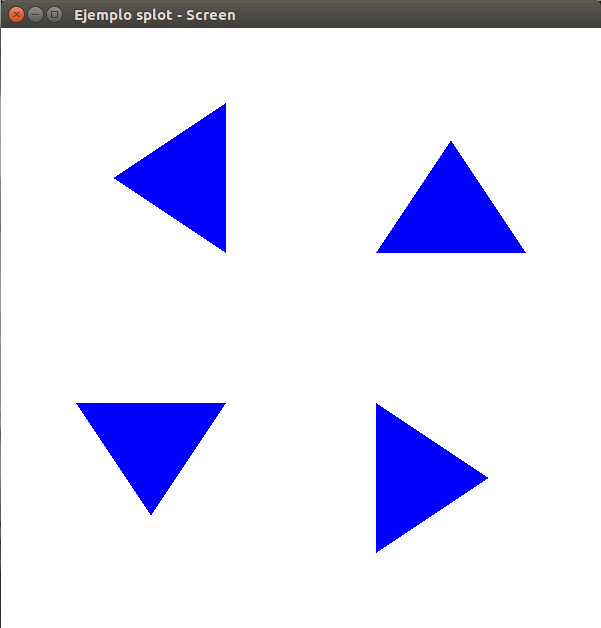
\includegraphics[scale = 0.5]{4.png}
  \caption{Resultados}
 \end{figure}
 
  \item \textbf{Utilizando sus propias funciones}
  
  A todas las funciones de los laboratorios pasados se le han unido dos más. La función \textit{drawTriangle} dibuja un triángulo a partir de tres puntos
  y retorna una matriz con los borde de éste. La función \textit{rotatePoint} recibe el punto que se quiere rotar, el punto eje por el cual se va a rotar, y 
  cuánto se va a rotar en grados.
  
  \textbf{Funciones}
  
  \begin{lstlisting}
Matrix drawTriangle(Point A, Point B, Point C, Window window){
    Matrix linea1 = drawLineXnpio(A,B,window);
    Matrix linea2 = drawLineXnpio(B,C,window);
    Matrix linea3 = drawLineXnpio(C,A,window);
    return linea1 + linea2 + linea3;
}

Point rotatePoint(Point punto, Point eje, float grados){
    Point res;
    float coseno = cos(grados*PI/180.0);
    float seno = sin(grados*PI/180.0);
    res.x = coseno * punto.x - seno * punto.y + eje.x * (1 - coseno) + eje.y * seno;
    res.y = seno * punto.x + coseno * punto.y + eje.y * (1 - coseno) - eje.x * seno;
    return res;
}
  \end{lstlisting}
  
  \textbf{main.cpp}
  
  \begin{lstlisting}
#include <GL/glut.h>
#include "primitivas.h"

Window window;

void init(){
	glClearColor(1.0,1.0,1.0,1.0);
	glMatrixMode(GL_PROJECTION);
	gluOrtho2D(0,600.0,0,600.0);
	glMatrixMode(GL_MODELVIEW);
}

void displayFcn(){
	Point A; A.x = 200; A.y = 300;
	Point B; B.x = 400; B.y = 400;
	Point C; C.x = 400; C.y = 200;
	Point eje; eje.x = 300; eje.y = 300;
	glClear(GL_COLOR_BUFFER_BIT);
	glColor3f(0.0,0.0,1.0);
	glViewport(0,300,300,300);
	Matrix triangle1 = drawTriangle(A, B, C, window);
	fillFigureScanLine(triangle1, AZUL);
	A = rotatePoint(A, eje, 90);
	B = rotatePoint(B, eje, 90);
	C = rotatePoint(C, eje, 90);
	glViewport(0,0,300,300);
	Matrix triangle2 = drawTriangle(A, B, C, window);
	fillFigureScanLine(triangle2, AZUL);
	A = rotatePoint(A, eje, 90);
	B = rotatePoint(B, eje, 90);
	C = rotatePoint(C, eje, 90);
	glViewport(300,0,300,300);
	Matrix triangle3 = drawTriangle(A, B, C, window);
	fillFigureScanLine(triangle3, AZUL);
	A = rotatePoint(A, eje, 90);
	B = rotatePoint(B, eje, 90);
	C = rotatePoint(C, eje, 90);
	glViewport(300,300,300,300);
	Matrix triangle4 = drawTriangle(A, B, C, window);
	fillFigureScanLine(triangle4, AZUL);
	glFlush();
}

int main(int argc, char ** argv){
	window.height = 600;
	window.width = 600;
	glutInit(&argc, argv);
	glutInitDisplayMode(GLUT_RGB | GLUT_SINGLE);
	glutInitWindowPosition(50,50);
	glutInitWindowSize(600,600);
	glutCreateWindow("Ejemplo splot - Screen");
	init();
	glutDisplayFunc(displayFcn);
	glutMainLoop();
	return 0;
}
  \end{lstlisting}

  \begin{figure}[H]
   \centering
   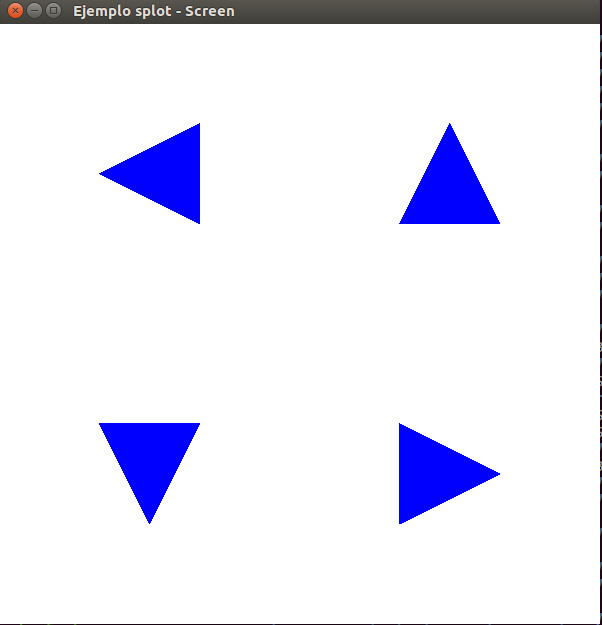
\includegraphics[scale = 0.5]{5.png}
   \caption{Resultados}
  \end{figure}

  \end{enumerate}
  
  \item \textbf{Un triángulo está definido por los puntos: (5,6),(7,8) y (3,7). Tiene un
  desface con respecto al origen de (2,1). Grafique el triángulo con un giro de 90
  grados y una simetría axial respecto a la horizontal.}
  
  Se dibuja una plano cartesiano y se convierten los puntos según las coordenadas de la ventana. Los triángulos se dibujan de la siguiente forma:
  \begin{itemize}
   \item El triángulo rojo es el original.
   \item El triángulo azul es con el desenfoque aplicado.
   \item El triángulo violeta es con la rotación aplicada.
   \item El triángulo magenta es el final.
  \end{itemize}
  
  \begin{lstlisting}
#include <GL/glut.h>
#include "primitivas.h"

Window window;

Point origen;

void init(){
	glClearColor(1.0,1.0,1.0,1.0);
	glMatrixMode(GL_PROJECTION);
	gluOrtho2D(0,600.0,0,600.0);
	glMatrixMode(GL_MODELVIEW);
}

Point convertirPunto(Point punto){
	int despl = 20;
	Point res;
	res.x = origen.x + despl * punto.x;
	res.y = origen.y + despl * punto.y;
	return res;
}

void displayFcn(){
	glClear(GL_COLOR_BUFFER_BIT);
	glColor3f(0.0,0.0,0.0);
	Point ejeX1; ejeX1.x = 20; ejeX1.y = 300;
	Point ejeX2; ejeX2.x = 580; ejeX2.y = 300;
	Point ejeY1; ejeY1.x = 300; ejeY1.y = 20;
	Point ejeY2; ejeY2.x = 300; ejeY2.y = 580;
	drawLineXnpio(ejeX1, ejeX2, window);
	drawLineXnpio(ejeY1, ejeY2, window);
	glBegin(GL_POINTS);	
		glVertex2f(origen.x, origen.y);
	glEnd();
	Point A; A.x = 5; A.y = 6;
	Point B; B.x = 7; B.y = 8;
	Point C; C.x = 3; C.y = 7;
	Point A_2 = convertirPunto(A);
	Point B_2 = convertirPunto(B);
	Point C_2 = convertirPunto(C);
	changeColor(ROJO);
	drawTriangle(A_2, B_2, C_2, window);
	Point eje; eje.x = 2; eje.y = 2;
	A.x += eje.x; A.y += eje.y;
	B.x += eje.x; B.y += eje.y;
	C.x += eje.x; B.y += eje.y;
	A_2 = convertirPunto(A);
	B_2 = convertirPunto(B);
	C_2 = convertirPunto(C);
	changeColor(AZUL);
	drawTriangle(A_2, B_2, C_2, window);
	A = rotatePoint(A, eje, 90);
	B = rotatePoint(B, eje, 90);
	C = rotatePoint(C, eje, 90);
	A_2 = convertirPunto(A);
	B_2 = convertirPunto(B);
	C_2 = convertirPunto(C);
	changeColor(VIOLETA);
	drawTriangle(A_2, B_2, C_2, window);
	A.y = -A.y;
	B.y = -B.y;
	C.y = -C.y;
	A_2 = convertirPunto(A);
	B_2 = convertirPunto(B);
	C_2 = convertirPunto(C);
	changeColor(MAGENTA);
	drawTriangle(A_2, B_2, C_2, window);
	glFlush();
}

int main(int argc, char ** argv){
	origen.x = 300; origen.y = 300;
	window.height = 600;
	window.width = 600;
	glutInit(&argc, argv);
	glutInitDisplayMode(GLUT_RGB | GLUT_SINGLE);
	glutInitWindowPosition(50,50);
	glutInitWindowSize(600,600);
	glutCreateWindow("Ejemplo splot - Screen");
	init();
	glutDisplayFunc(displayFcn);
	glutMainLoop();
	return 0;
}
  \end{lstlisting}

  \begin{figure}[H]
   \centering
   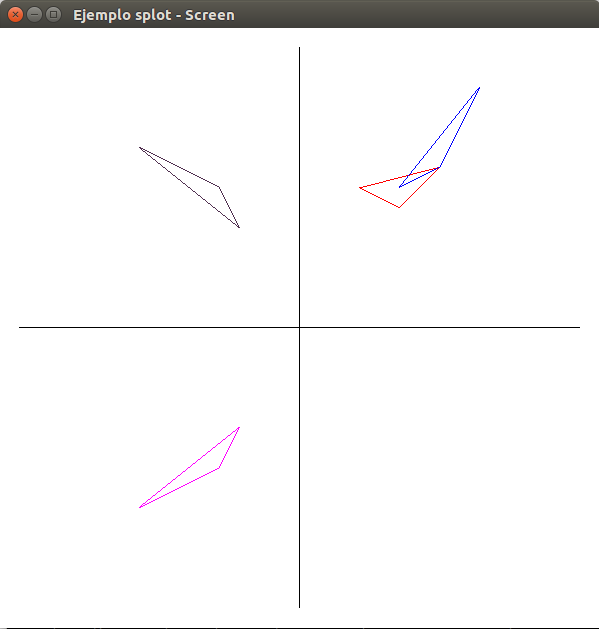
\includegraphics[scale = 0.5]{6.png}
   \caption{Resultado}
  \end{figure}



 
\end{enumerate}


\end{document}

